\documentclass[10pt]{article}
\usepackage[a4paper,hmargin=2cm,vmargin=1.8cm]{geometry}
\linespread{0.97}
\usepackage{amsmath,amssymb}
\usepackage[T1]{fontenc}
\usepackage{lmodern}
\usepackage{graphicx}
\usepackage{booktabs}
\usepackage{array}
\usepackage{tikz}
% Online Resource layout: captions in the journal's style (small type, label then a quad, caption above tables
% with a gap to the top rule), supplement numbering S1, S2, ... so no table or figure shares a number with the
% main paper, and more room between floats and the surrounding text
\usepackage[font=small,labelfont=bf,labelsep=quad,skip=6pt]{caption}
\captionsetup[table]{position=top}
\captionsetup[figure]{name=Fig.}
\renewcommand{\thetable}{S\arabic{table}}
\renewcommand{\thefigure}{S\arabic{figure}}
\renewcommand{\topfraction}{0.9}
\renewcommand{\bottomfraction}{0.8}
\renewcommand{\textfraction}{0.07}
\renewcommand{\floatpagefraction}{0.85}
\setcounter{topnumber}{3}
\setcounter{totalnumber}{5}
\setlength{\intextsep}{10pt plus 3pt minus 2pt}
\setlength{\textfloatsep}{12pt plus 3pt minus 2pt}
\setlength{\floatsep}{10pt plus 3pt minus 2pt}
\usetikzlibrary{arrows.meta,fit,shapes.symbols,shapes.geometric,positioning,calc}
\title{Online Resource 1\\[4pt]\large Supplementary material for the article ``AXIOM: A Shared Controller for Scalable Multi-Agent 5G Slice Admission''\\[2pt]\normalsize Wireless Personal Communications}
\author{Manoj Prasad Kunasegran, Wai Leong Pang, Swee King Phang\\[4pt]
\small Corresponding author Wai Leong Pang, \texttt{waileong.pang@taylors.edu.my}\\
\small School of Engineering, Faculty of Innovation and Technology, Taylor's University,\\
\small 47500 Subang Jaya, Selangor, Malaysia}
\date{}
\pdfinfo{/Title (Online Resource 1: AXIOM: A Shared Controller for Scalable Multi-Agent 5G Slice Admission)
  /Author (Manoj Prasad Kunasegran, Wai Leong Pang, Swee King Phang) /Subject (Wireless Personal Communications)}
\begin{document}
\maketitle

\section*{S1. Overview}
This supplement gives the detail behind the main paper's results for AXIOM, short for Adaptive Cross-cell Integrated Orchestration of Multi-slice admission, without repeating what the main paper states. Every pass criterion was fixed in a pre-registration committed before the run it judged, and Table~\ref{tab:s-acronyms} lists the acronyms used here.

\begin{table}[!htbp]
\caption{Acronyms used in this supplement}
\label{tab:s-acronyms}
\centering
\footnotesize
{\setlength{\tabcolsep}{3pt}
\begin{tabular}{@{}l>{\raggedright\arraybackslash}p{0.21\textwidth}@{\hspace{1em}}l>{\raggedright\arraybackslash}p{0.21\textwidth}@{\hspace{1em}}l>{\raggedright\arraybackslash}p{0.21\textwidth}@{}}
\toprule
Acronym & Meaning & Acronym & Meaning & Acronym & Meaning \\
\midrule
CI & Confidence interval & gNB & gNodeB, the 5G base station & RF & Radio frequency \\
CPU & Central processing unit & GPU & Graphics processing unit & RIC & RAN Intelligent Controller \\
DP & Differential privacy & IQM & Interquartile mean & SDR & Software-defined radio \\
DP-SGD & Differentially private stochastic gradient descent & MAPPO & Multi-agent proximal policy optimisation & SLA & Service Level Agreement \\
DQN & Deep Q-network & MLP & Multi-layer perceptron & TDD & Time-division duplex \\
DQN-I & Independent per-gNB deep Q-networks & mMTC & Massive Machine-Type Communication & UDP & User Datagram Protocol \\
DQN-SA & Single-agent deep Q-network & OAI & OpenAirInterface & UE & User equipment \\
eMBB & Enhanced Mobile Broadband & O-RAN & Open Radio Access Network & URLLC & Ultra-Reliable Low-Latency Communication \\
FedAvg & Federated averaging & PRB & Physical resource block & VDN & Value-decomposition network \\
GAT & Graph attention network & RAN & Radio Access Network &  &  \\
\bottomrule
\end{tabular}}
\end{table}

\section*{S2. Verification runs}
The fresh-seed runs of the main paper's Section 6.6 retrained every policy on seeds from 3000 onwards. In Env A AXIOM reached 98.2\% of the static rule's reward at three gNBs and at nineteen gNBs kept 95.6\% priority-slice compliance against 47.8\% to 65.5\% for the baselines. Of the nine failed checks, the four that concern AXIOM are small margins, and twenty-seed reruns did not reproduce two of them.

Fig.~\ref{fig:s-forest} sets each reported comparison with a learned baseline beside its fresh-seed counterpart. The three reported differences that fresh seeds do not keep all concern cluster-level compliance in Env B. AXIOM's deficits of 9.2 points to DQN-SA and 4.8 points to DQN-I at seven gNBs become 4.2 points and a 0.8-point lead. Its lead over MAPPO at nineteen gNBs falls to 2.9 points, and all three fresh CIs span zero.

\begin{figure}[!htbp]
\centering
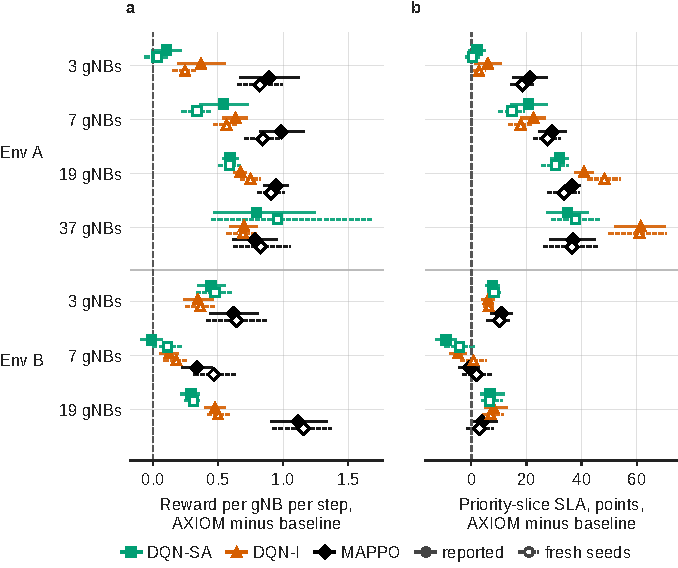
\includegraphics{figures/fig_forest.pdf}
\caption{AXIOM minus each learned baseline, with 95\% CIs. Solid lines and filled circles are the reported runs, dashed lines and hollow diamonds the fresh seeds. a, Reward per gNB. b, Cluster-level priority-slice compliance}
\label{fig:s-forest}
\end{figure}

Table~\ref{tab:s-rliable} gives the interquartile means and probabilities of improvement that Agarwal et al., cited in the main paper, recommend for evaluations with few runs, computed with rliable 1.2.0 on the main paper's pooled runs. The IQM drops the worst quarter of runs, where AXIOM's few collapses sit. AXIOM's IQM of priority-slice compliance in Env A is therefore 100.0\% at every size, against means of 93.7\% to 98.9\%, and the mean stays the more conservative summary for AXIOM. An independent implementation reproduces every IQM and every probability of improvement to within $10^{-6}$, and Fig.~\ref{fig:s-rliable} shows the fraction of runs above each compliance level.

\begin{table}[!htbp]
\caption{Interquartile means of reward per gNB per step and of priority-slice compliance, and the probability P that a run of AXIOM beats a run of each other policy, with ties counted as one half. Brackets give stratified bootstrap 95\% CIs over 10{,}000 resamples}
\label{tab:s-rliable}
\centering
\scriptsize
{\setlength{\tabcolsep}{3.5pt}
\begin{tabular}{@{}lccccc@{}}
\toprule
Policy & Runs & IQM reward per gNB & IQM priority SLA, \% & P, reward & P, priority SLA \\
\midrule
\multicolumn{6}{@{}l}{Env A, 3 gNBs} \\
\quad AXIOM & 30 & 4.266 [4.24, 4.29] & 100.0 [100.0, 100.0] & -- & -- \\
\quad DQN-SA & 30 & 4.197 [4.12, 4.24] & 99.5 [97.4, 100.0] & 0.68 [0.53, 0.81] & 0.68 [0.56, 0.79] \\
\quad DQN-I & 30 & 4.018 [3.80, 4.10] & 98.1 [92.4, 99.7] & 0.89 [0.80, 0.97] & 0.76 [0.65, 0.86] \\
\quad MAPPO & 30 & 3.378 [3.02, 3.72] & 77.4 [67.2, 87.7] & 0.92 [0.83, 0.99] & 0.92 [0.84, 0.98] \\
\quad Static rule & 30 & 4.269 [4.25, 4.29] & 100.0 [100.0, 100.0] & 0.47 [0.32, 0.62] & 0.45 [0.36, 0.53] \\
\midrule
\multicolumn{6}{@{}l}{Env A, 7 gNBs} \\
\quad AXIOM & 45 & 4.562 [4.52, 4.58] & 100.0 [99.7, 100.0] & -- & -- \\
\quad DQN-SA & 45 & 4.065 [3.95, 4.16] & 79.4 [72.9, 85.1] & 0.87 [0.78, 0.94] & 0.88 [0.79, 0.95] \\
\quad DQN-I & 45 & 3.849 [3.79, 3.92] & 73.3 [69.3, 77.7] & 0.96 [0.91, 1.00] & 0.94 [0.88, 0.99] \\
\quad MAPPO & 45 & 3.573 [3.33, 3.72] & 64.5 [60.4, 69.6] & 0.96 [0.92, 0.99] & 0.96 [0.91, 0.99] \\
\quad Static rule & 45 & 4.582 [4.57, 4.59] & 100.0 [100.0, 100.0] & 0.33 [0.22, 0.44] & 0.38 [0.29, 0.46] \\
\midrule
\multicolumn{6}{@{}l}{Env A, 19 gNBs} \\
\quad AXIOM & 90 & 4.743 [4.74, 4.75] & 100.0 [100.0, 100.0] & -- & -- \\
\quad DQN-SA & 90 & 4.129 [4.12, 4.14] & 66.8 [65.9, 67.6] & 0.95 [0.90, 0.99] & 0.96 [0.92, 0.99] \\
\quad DQN-I & 90 & 4.025 [4.00, 4.05] & 56.0 [52.6, 59.6] & 0.97 [0.94, 0.99] & 0.98 [0.96, 1.00] \\
\quad MAPPO & 90 & 3.778 [3.69, 3.86] & 58.4 [56.6, 60.7] & 0.99 [0.97, 1.00] & 0.98 [0.95, 0.99] \\
\quad Static rule & 90 & 4.749 [4.74, 4.76] & 100.0 [100.0, 100.0] & 0.44 [0.36, 0.52] & 0.44 [0.39, 0.49] \\
\midrule
\multicolumn{6}{@{}l}{Env A, 37 gNBs} \\
\quad AXIOM & 60 & 4.796 [4.78, 4.80] & 100.0 [99.2, 100.0] & -- & -- \\
\quad DQN-SA & 30 & 4.218 [4.19, 4.23] & 61.5 [60.3, 62.9] & 0.94 [0.88, 0.98] & 0.92 [0.85, 0.97] \\
\quad DQN-I & 30 & 3.999 [3.94, 4.07] & 26.0 [19.3, 37.7] & 0.98 [0.96, 1.00] & 0.98 [0.95, 1.00] \\
\quad MAPPO & 30 & 3.968 [3.83, 4.10] & 54.3 [48.8, 61.3] & 0.97 [0.93, 0.99] & 0.95 [0.90, 0.98] \\
\quad Static rule & 30 & 4.799 [4.80, 4.80] & 100.0 [100.0, 100.0] & 0.41 [0.29, 0.53] & 0.42 [0.35, 0.51] \\
\midrule
\multicolumn{6}{@{}l}{Env B, 3 gNBs} \\
\quad AXIOM & 30 & 2.940 [2.87, 3.02] & 65.2 [63.6, 66.9] & -- & -- \\
\quad DQN-SA & 30 & 2.558 [2.41, 2.64] & 58.2 [55.9, 60.2] & 0.94 [0.87, 0.98] & 0.87 [0.77, 0.95] \\
\quad DQN-I & 30 & 2.625 [2.50, 2.73] & 59.4 [57.8, 60.7] & 0.84 [0.73, 0.93] & 0.84 [0.73, 0.94] \\
\quad MAPPO & 30 & 2.361 [2.14, 2.55] & 54.6 [50.3, 58.6] & 0.92 [0.83, 0.98] & 0.86 [0.75, 0.94] \\
\quad Static rule & 30 & 2.110 [1.97, 2.24] & 49.4 [46.9, 51.7] & 0.99 [0.98, 1.00] & 0.99 [0.96, 1.00] \\
\quad Tuned rule & 30 & 3.067 [3.02, 3.12] & 67.5 [66.8, 68.3] & 0.27 [0.15, 0.40] & 0.31 [0.18, 0.45] \\
\midrule
\multicolumn{6}{@{}l}{Env B, 7 gNBs} \\
\quad AXIOM & 45 & 3.338 [3.31, 3.38] & 33.3 [32.4, 35.1] & -- & -- \\
\quad DQN-SA & 45 & 3.406 [3.33, 3.47] & 45.7 [41.6, 49.4] & 0.43 [0.31, 0.56] & 0.23 [0.13, 0.34] \\
\quad DQN-I & 45 & 3.225 [3.18, 3.28] & 39.3 [37.0, 41.8] & 0.72 [0.61, 0.83] & 0.27 [0.16, 0.38] \\
\quad MAPPO & 45 & 3.018 [2.92, 3.13] & 33.0 [29.0, 38.2] & 0.79 [0.69, 0.89] & 0.58 [0.44, 0.71] \\
\quad Static rule & 45 & 3.354 [3.33, 3.39] & 33.2 [32.3, 34.3] & 0.45 [0.33, 0.57] & 0.52 [0.40, 0.64] \\
\quad Tuned rule & 45 & 3.896 [3.88, 3.91] & 60.4 [60.1, 60.8] & 0.00 [0.00, 0.00] & 0.00 [0.00, 0.00] \\
\midrule
\multicolumn{6}{@{}l}{Env B, 19 gNBs} \\
\quad AXIOM & 15 & 4.269 [4.18, 4.29] & 22.6 [21.7, 24.1] & -- & -- \\
\quad DQN-SA & 15 & 3.931 [3.92, 3.95] & 17.9 [17.7, 18.2] & 0.95 [0.83, 1.00] & 0.98 [0.91, 1.00] \\
\quad DQN-I & 15 & 3.755 [3.69, 3.82] & 16.5 [15.9, 17.4] & 1.00 [0.97, 1.00] & 0.99 [0.96, 1.00] \\
\quad MAPPO & 15 & 3.121 [2.96, 3.29] & 19.9 [19.4, 22.1] & 1.00 [1.00, 1.00] & 0.77 [0.56, 0.94] \\
\quad Static rule & 15 & 4.294 [4.28, 4.31] & 22.8 [22.1, 23.6] & 0.31 [0.13, 0.51] & 0.46 [0.26, 0.68] \\
\quad Tuned rule & 15 & 4.427 [4.41, 4.44] & 55.6 [55.2, 56.1] & 0.00 [0.00, 0.00] & 0.05 [0.00, 0.17] \\
\bottomrule
\end{tabular}}
\end{table}

\begin{figure}[!htbp]
\centering
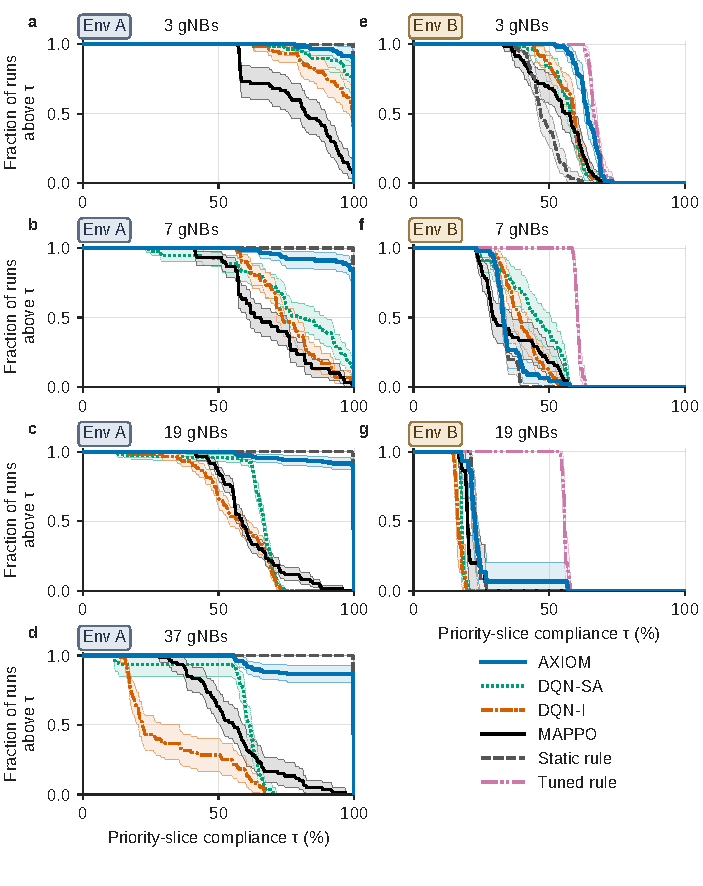
\includegraphics{figures/fig_rliable.pdf}
\caption{Performance profiles of priority-slice compliance, the fraction of runs above each level $\tau$. Shaded bands are stratified bootstrap 95\% CIs. a to d, Env A at 3, 7, 19, and 37 gNBs. e to g, Env B at 3, 7, and 19 gNBs}
\label{fig:s-rliable}
\end{figure}

\section*{S3. Live testbed}
Every live measurement comes from the single-host, software-radio O-RAN stack of Fig.~\ref{fig:testbed}, which runs without a near-real-time RIC because the ORANSlice fork cited in the main paper applies slicing control through a lightweight UDP E2 agent. AXIOM itself is not deployed there, since its multi-gNB policy needs at least two live gNBs and our two-gNB attempt did not sustain traffic. A single-agent DQN checkpoint instead exercises the control path, PRB-ratio actuation, and real-time inference at one and at two UEs per slice. A capacity probe showed every slice served at essentially 100\% of offered demand, so the rig never ran short of capacity and shows the pipeline working, not admission under contention. The rig starts the Open5GS core with Docker Compose and the gNB with \texttt{nr-softmodem} on the rfsim radio, and attaches up to six UEs. It runs the checkpoint through the UDP E2 agent on ports 6600 and 6655. Drive iperf3 UDP traffic on every slice to reproduce its load. A scheduler-configuration error that granted fewer PRBs than the gNB scheduler's five-PRB floor was fixed at the root. Instrumentation then confirmed zero below-floor grants across more than 100{,}000 readings.

\begin{figure}[!htbp]
\centering
\resizebox{0.9\textwidth}{!}{%
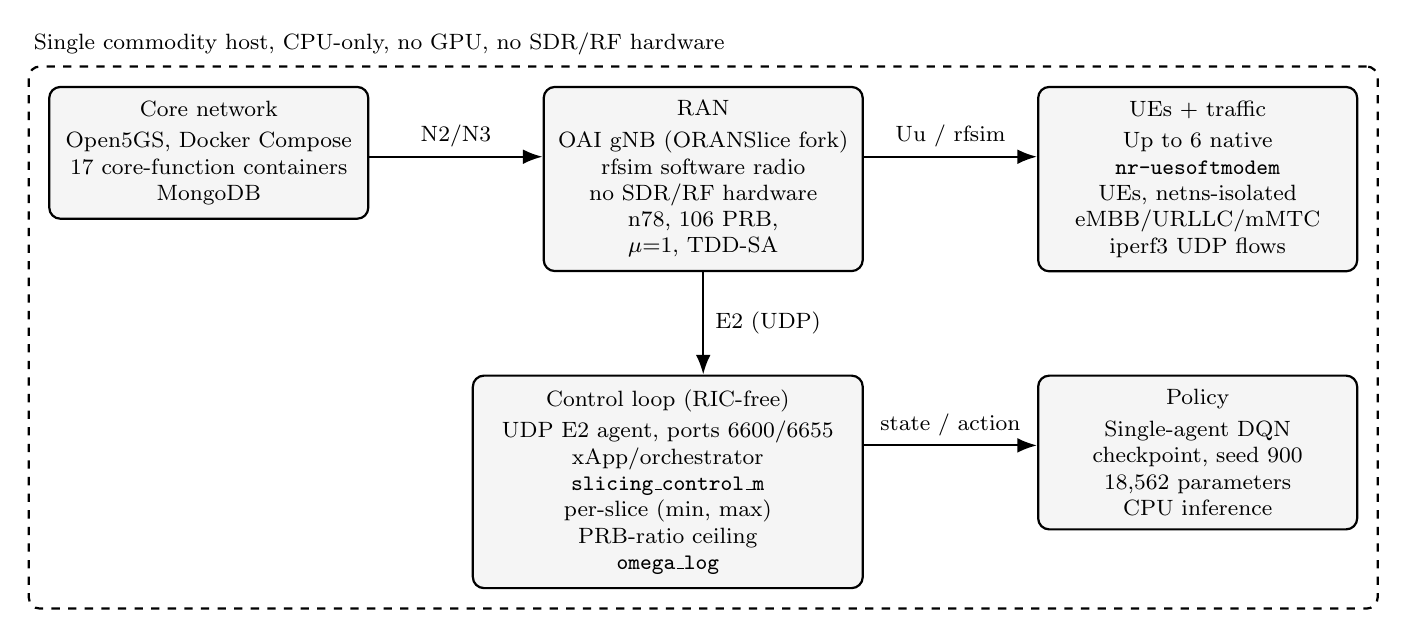
\begin{tikzpicture}[
  block/.style={draw, thick, rounded corners, align=center, fill=gray!8,
                font=\footnotesize, inner sep=5pt, text width=3.7cm},
  arr/.style={-{Latex[length=2.5mm]}, thick},
  lbl/.style={font=\footnotesize, inner sep=1pt}
]
\node[block, anchor=north] (core) at (0,0)
  {Core network\\[2pt]
   Open5GS, Docker Compose\\
   17 core-function containers\\
   MongoDB};
\node[block, anchor=north west] (ran) at ($(core.north east)+(2.2,0)$)
  {RAN\\[2pt]
   OAI gNB (ORANSlice fork)\\
   rfsim software radio\\
   no SDR/RF hardware\\
   n78, 106 PRB, $\mu{=}1$, TDD-SA};
\node[block, anchor=north west] (ues) at ($(ran.north east)+(2.2,0)$)
  {UEs + traffic\\[2pt]
   Up to 6 native \texttt{nr-uesoftmodem} UEs, netns-isolated\\
   eMBB/URLLC/mMTC iperf3 UDP flows};
\node[block, anchor=north east, text width=4.6cm] (ctrl) at ($(ran.south east)+(0,-1.3)$)
  {Control loop (RIC-free)\\[2pt]
   UDP E2 agent, ports 6600/6655\\
   xApp/orchestrator \texttt{slicing\_control\_m}\\
   per-slice (min, max) PRB-ratio ceiling\\
   \texttt{omega\_log}};
\node[block, anchor=north] (policy) at (ues.south |- ctrl.north)
  {Policy\\[2pt]
   Single-agent DQN checkpoint, seed 900\\
   18{,}562 parameters\\
   CPU inference};
\draw[arr] ($(core.north east)+(0,-0.9)$) -- ($(ran.north west)+(0,-0.9)$) node[lbl, midway, above=2pt] {N2/N3};
\draw[arr] ($(ran.north east)+(0,-0.9)$) -- ($(ues.north west)+(0,-0.9)$) node[lbl, midway, above=2pt] {Uu / rfsim};
\draw[arr] (ran.south) -- (ran.south |- ctrl.north) node[lbl, midway, right=3pt] {E2 (UDP)};
\draw[arr] ($(ctrl.north east)+(0,-0.9)$) -- ($(policy.north west)+(0,-0.9)$) node[lbl, midway, above=2pt] {state / action};
\node[draw, thick, dashed, rounded corners, inner sep=7pt, fit=(core)(ran)(ues)(ctrl)(policy)] (host) {};
\node[font=\footnotesize, anchor=south west, inner sep=2pt] at ($(host.north west)+(0,0.05)$)
  {Single commodity host, CPU-only, no GPU, no SDR/RF hardware};
\end{tikzpicture}%
}
\caption{Real testbed stack, a single-host, software-radio rfsim,
RIC-free O-RAN deployment distinguished from software-defined-radio hardware-in-the-loop
testbeds. Every block and label is a measured or configured value from
this rig}
\label{fig:testbed}
\end{figure}

\section*{S4. Setup, safeguards, and analysis plans}
A sensitivity study repeats the learned policies and the static rule in Env A on 10 seeds at 102\% and 107\% of the nominal load. It also changes the slice weights, lowering eMBB from 3.5 to 2.5 and raising mMTC from 0.3 to 0.6. A second repeats AXIOM in Env B on 10 seeds at learning rates of $3{\times}10^{-4}$ and $3{\times}10^{-3}$ and with an encoder twice as wide. The federated campaign runs in Env A on seeds 900 to 909, with noise multipliers $\sigma \in \{0, 0.5, 1, 2, 4\}$ and a replication on seeds 1000 to 1009. Each round runs 50 local steps of federated averaging (FedAvg) with a gradient-clip norm of $1.0$. A validation screen checks every trained checkpoint before evaluation. Each plays five greedy episodes on its own training stream and fails if it blocks no request or if fewer than 90\% of its blocks target mMTC. In Env B, where the reward-optimal policy also sheds eMBB, the no-blocking criterion is the primary screen. The Env B constants, AXIOM's learning rate, and its skip connection were all chosen on pilot seeds 2000 to 2009.

AXIOM's encoder is a graph-attention network over the gNB graph. Each gNB forms its own feature row $\mathbf{x}_i$ of PRB-used ratio, congestion level, and normalised queue length, and a two-layer network with $H{=}4$ heads produces one embedding per gNB. Each head $h$ uses a learned source vector $\mathbf{a}_s^{h}$ and destination vector $\mathbf{a}_d^{h}$ on the shared projection $\mathbf{W}^{h}$. Here $\mathrm{LeakyReLU}$, the leaky rectified linear unit, has slope $0.2$ for negative inputs, and $\mathcal{N}_i$ is the set of neighbours of node $i$,
\begin{equation}
\varepsilon_{ij}^{h}=\mathrm{LeakyReLU}\big(\mathbf{a}_s^{h\top} \mathbf{W}^{h} \mathbf{x}_i + \mathbf{a}_d^{h\top} \mathbf{W}^{h} \mathbf{x}_j\big),
\qquad
\alpha_{ij}^{h}=\frac{\exp\varepsilon_{ij}^{h}}{\sum_{l\in\mathcal{N}_i}\exp\varepsilon_{il}^{h}}.
\end{equation}
Hidden layers concatenate the $H$ heads under an exponential linear unit, the final layer averages them, and a per-layer normalisation $\mathrm{LN}(\cdot)$ rescales each embedding to zero mean and unit variance,
\begin{equation}
\mathbf{z}_i=\mathrm{LN}\!\Big(\tfrac{1}{H}\textstyle\sum_{h=1}^{H}\sum_{j\in\mathcal{N}_i}\alpha_{ij}^{h}\,\mathbf{W}^{h} \mathbf{x}_j\Big).
\end{equation}
An earlier variant fed each gNB's summed per-request values into a QMIX-style mixer, and its mean training loss diverged from about 76 to about 409. Treating each request as its own sample removed that dependence.

In the federated variant each client clips its minibatch gradient to norm $C_{\text{dp}}$ and adds Gaussian noise of standard deviation $\sigma C_{\text{dp}}$. Zero-concentrated differential privacy composes this over the $m$ noisy steps a client takes,
\begin{equation}
\label{eq:zcdp}
\rho=\frac{2m}{\sigma^{2}},\qquad
\varepsilon(\delta)=\rho+2\sqrt{\rho\ln(1/\delta)}.
\end{equation}
We credit no amplification by subsampling, because minibatches come from a replay buffer that reuses records, so the bound is conservative.

The trivial-policy check of the main paper's Section 5.1 rests on these numbers. In our first simulator, where every slice was served against its own ceiling, accepting every request earned 14.45 reward per step and kept URLLC and eMBB at 100\% SLA compliance. Over the same 30 held-out seeds in the shared-budget simulator, accepting every request now earns 9.89 reward per step and lets eMBB compliance fall to 56.8\%, whereas shedding every mMTC request earns 12.84.

The main campaign reuses Env A results of DQN-SA, DQN-I, and the static rule from an earlier rerun, M63. They cover three gNBs on the primary and replication seeds, the sensitivity study, seven gNBs, and 15 of the 30 seeds at nineteen gNBs. Two development stages are disclosed, although neither changed a reported result. A protocol, M67, tested checkpoint selection and both encoders on new seeds and left AXIOM unchanged, and exploratory probes on seeds 900 to 904 suggested the load-shift effect of Section S7 before its reported runs. M92, the zero-shot transfer of Section S6, and M94, the distillation of Section S7, were each committed before their runs. M93, the summary of Section S2, reanalyses stored logs only and has no plan of its own. Section 5.2 of the main paper describes how an artificial intelligence assistant was used in this work.

\section*{S5. Three gNBs, ablations, federation, and disruption}
The MLP variant reads only a gNB's own features. In Env A it ties AXIOM, which earns 0.058 more reward per step at three gNBs with 95\% CI [$-$0.17, 0.26] and 0.31 more at nineteen gNBs on the ring layout, with 7 of 12 seeds tied. A disjoint replication on seeds 1000 to 1009 is stronger for AXIOM. There it earns 1.083, 0.799, and 3.806 more reward per step than DQN-SA, DQN-I, and MAPPO, and pooled over all 40 seeds its margins over the three baselines are 0.504, 1.032, and 2.965 reward per step at Holm-adjusted $p\leq0.002$.

A grid of 24 MAPPO configurations raised MAPPO from 60.6\% to 69.6\% priority-slice compliance at nineteen gNBs on the ring layout, and AXIOM still beats it by 1.25 to 16.18 reward per step at Holm-adjusted $p<0.001$. With its initialisation properly seeded, DQN-SA keeps 80.3\% and 63.9\% priority-slice compliance at seven and nineteen gNBs, and AXIOM beats it under every layout at Holm-adjusted $p\leq0.035$.

Fig.~\ref{fig:m3-privacy} shows the federated campaign. With federation and no noise, mean reward per step on the ten shared seeds is 12.356 for centralised AXIOM and 11.929 for the federated variant. That is a difference of $+0.427$ with 95\% CI [$-$0.54, 1.51] and $p=0.65$, so federation shows no significant cost on these seeds. Each client takes 17{,}969 noisy steps over its training run. At $\delta{=}10^{-5}$ Eq.~\eqref{eq:zcdp} then gives $\varepsilon$ of about 146{,}000, 37{,}000, 9{,}600, and 2{,}600 for $\sigma$ of 0.5, 1, 2, and 4, so a useful guarantee would need noise on the roughly 360 per-round model updates instead.

\begin{figure}[!htbp]
\centering
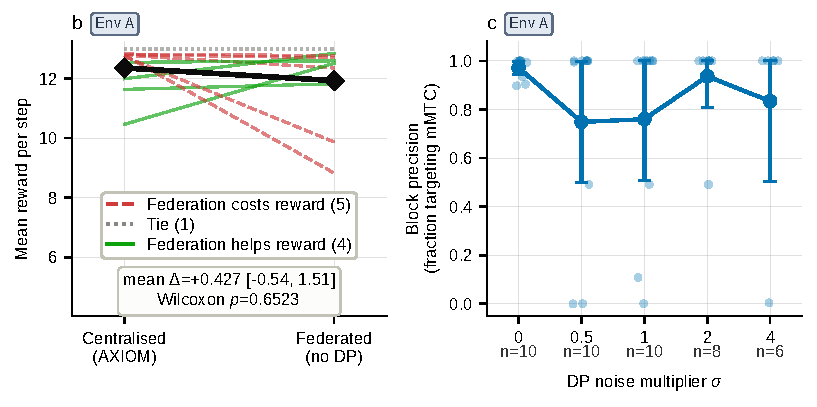
\includegraphics{figures/fig4_m3_privacy.pdf}
\caption{Federated campaign in Env A, 10 seeds. a, Paired per-seed federation
cost on mean reward per step, not significant at $p=0.65$. b, Block precision
versus DP noise multiplier $\sigma$, over the seeds that block}
\label{fig:m3-privacy}
\end{figure}

Each policy's frozen Env A checkpoint also faced three disruptions. A gNB dropout forces one gNB to reject everything, a demand spike multiplies the arrival rate, and an agent churn swaps one gNB's decisions for an untrained copy. Dropout and churn windows last 10\%, 30\%, or 60\% of the episode. Spikes multiply arrivals by 2, 4, or 8. Fig.~\ref{fig:m4-disruption} shows the reward each policy keeps, normalised by each step's pending-request count.

\begin{figure}[!htbp]
\centering
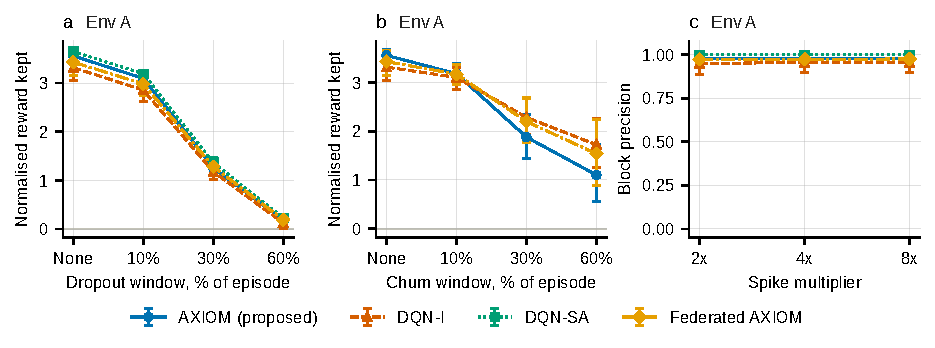
\includegraphics{figures/fig5_m4_disruption.pdf}
\caption{Disruption campaign, 10 seeds per policy, 95\% CIs. a, b, Normalised
reward kept under dropout and churn, with the undisrupted level at the tick marked None.
c, Block precision under demand spikes}
\label{fig:m4-disruption}
\end{figure}

\section*{S6. Scaling to thirty-seven gNBs and stronger baselines}
In the gate map of the main paper's thirty-seven-gNB cluster, DQN-SA leaves every admission gate open at 0.93 to 0.95 and DQN-I closes the mMTC gate only to 0.94. MAPPO there partly closes the eMBB gate to 0.80 but leaves mMTC open at 0.51. At seven gNBs AXIOM keeps URLLC and eMBB at 99.8\% and 94.4\%, against 87.0\% to 94.2\% and 48.4\% to 61.0\% for the baselines, and at thirty-seven at 96.7\% and 90.7\%. The thirty-seven-gNB configuration extends the smaller ones, with 37 arrivals per step and at most 148 pending requests, and Table~\ref{tab:s-n37} lists every policy. AXIOM's six collapsed runs keep 59\% to 65\% priority-slice compliance, while its other runs keep 96.9\% to 98.1\% on average under each layout.

\begin{table}[!htbp]
\caption{Env A with thirty-seven gNBs, reported and fresh seeds. Priority-slice compliance is the mean of URLLC and eMBB compliance, and collapse counts policies that accept every request}
\label{tab:s-n37}
\centering
\footnotesize
\begin{tabular}{lcccccc}
\toprule
Policy & Runs & URLLC & eMBB & Priority SLA & Reward & Collapsed \\
\midrule
AXIOM, hex & 30 & 97.4\% & 89.8\% & 93.6\% & 174.20 & 3 \\
AXIOM, ring & 15 & 93.7\% & 92.6\% & 93.2\% & 173.51 & 2 \\
AXIOM, fully-connected & 15 & 98.4\% & 90.4\% & 94.4\% & 174.44 & 1 \\
DQN-SA & 30 & 73.3\% & 44.1\% & 58.7\% & 144.70 & 26 \\
DQN-I & 30 & 38.6\% & 25.7\% & 32.1\% & 148.35 & 3 \\
MAPPO & 30 & 67.8\% & 45.6\% & 56.7\% & 145.25 & 0 \\
Static rule & 30 & 100.0\% & 100.0\% & 99.98\% & 177.58 & 0 \\
\midrule
\multicolumn{7}{@{}l}{Fresh seeds 6100 to 6119, hex layout} \\
AXIOM & 20 & 95.4\% & 94.7\% & 95.1\% & 174.67 & 1 \\
DQN-SA & 20 & 71.6\% & 43.1\% & 57.4\% & 139.20 & 18 \\
DQN-I & 20 & 42.0\% & 26.1\% & 34.1\% & 149.04 & 2 \\
MAPPO & 20 & 70.1\% & 47.0\% & 58.5\% & 144.04 & 0 \\
Static rule & 20 & 100.0\% & 100.0\% & 99.97\% & 177.68 & 0 \\
\bottomrule
\end{tabular}
\end{table}

The DQN baselines were also tuned on pilot seeds over learning rates from $10^{-4}$ to $10^{-3}$ and minibatches of 16 and 64, as Table~\ref{tab:s-tuned} lists. No tuned baseline exceeds the accept-all floor at either size, and AXIOM beats each one on compliance and reward in every setting, winning 26 to 30 of 30 seeds at Holm-adjusted $p<0.001$. VDN, which trains DQN-I's per-gNB networks on one joint target, ties AXIOM at three gNBs but falls behind at nineteen, as Table~\ref{tab:s-vdn} shows.

\begin{table}[!htbp]
\caption{DQN baselines tuned on pilot seeds, Env A, 30 hex seeds. LR is the learning rate, batch the minibatch size, and Before the priority-slice compliance before tuning}
\label{tab:s-tuned}
\centering
\footnotesize
\setlength{\tabcolsep}{4pt}
\begin{tabular}{lcccccc}
\toprule
Baseline & gNBs & LR, batch & Priority SLA & Before & Reward & Collapsed \\
\midrule
DQN-SA & 19 & $10^{-4}$, 16 & 67.1\% & 65.3\% & 78.55 & 30 \\
DQN-I & 19 & $3{\times}10^{-4}$, 64 & 59.1\% & 56.4\% & 77.07 & 11 \\
DQN-SA & 37 & $10^{-3}$, 16, unchanged & 58.7\% & 58.7\% & 144.70 & 26 \\
DQN-I & 37 & $10^{-4}$, 64 & 45.5\% & 32.1\% & 150.42 & 18 \\
\bottomrule
\end{tabular}
\end{table}

\begin{table}[!htbp]
\caption{VDN against AXIOM and DQN-I, reward per step and priority-slice compliance, 30 seeds per setting}
\label{tab:s-vdn}
\centering
\footnotesize
\setlength{\tabcolsep}{3pt}
\begin{tabular}{lcccccc}
\toprule
Setting & VDN & AXIOM & DQN-I & VDN SLA & AXIOM SLA & DQN-I SLA \\
\midrule
Env A, 3 gNBs & 12.664 & 12.698 & 11.587 & 99.0\% & 98.9\% & 92.9\% \\
Env B, 3 gNBs & 8.552 & 8.832 & 7.794 & 62.5\% & 65.1\% & 59.0\% \\
Env A, 19 gNBs, hex & 86.428 & 89.161 & 76.388 & 83.4\% & 97.0\% & 56.4\% \\
\bottomrule
\end{tabular}
\end{table}

Fig.~\ref{fig:s-layouts} gives the per-layout view of the Env A scaling results that the main paper pools over layouts.

\begin{figure}[!htbp]
\centering
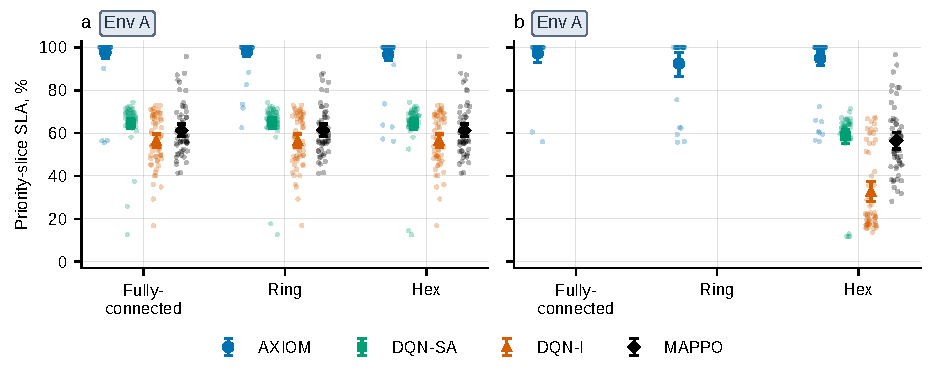
\includegraphics{figures/fig14_layouts.pdf}
\caption{Env A priority-slice compliance by layout, per-seed points behind the mean and 95\% CI. a, Nineteen gNBs, 30 seeds per layout. b, Thirty-seven gNBs, where the baselines never read the layout and ran once, on the hex seeds}
\label{fig:s-layouts}
\end{figure}

The transfer run of the main paper's Section 6.2, M92, also covered AXIOM's MLP variant in Env B. The stored network also holds a mixer left from an earlier training design. No current loss uses it and its input grows with the cluster, so the loader copies every other parameter and AXIOM keeps its 7,782 execution parameters. Before the plan was committed, six stored evaluations were rerun through the same loader at their own size, and each reproduced exactly. Table~\ref{tab:s-transfer} adds CIs, reward, and collapses to the main paper's transfer table. In Env B the endpoint is per-gNB compliance, because cluster-level compliance, which needs all nineteen gNBs to comply at once, stays between 18\% and 36\% for every policy there. Graph attention again adds nothing measurable, since AXIOM transferred from seven gNBs keeps 0.80 points more per-gNB compliance than its MLP variant, with 95\% CI [$-$2.23, 3.81] and $p=0.72$. On the fully-connected layout at nineteen gNBs, AXIOM trained at that size makes exactly the static rule's decisions on every seed, so the transferred policy trails it by 0.10 reward per gNB, at $p=0.068$.

\begin{table}[!htbp]
\caption{Zero-shot transfer from seven gNBs on 15 paired seeds, priority-slice compliance with 95\% CIs, reward per gNB per step, and collapsed runs. The main paper's transfer table gives the rule references}
\label{tab:s-transfer}
\centering
\scriptsize
{\setlength{\tabcolsep}{3pt}
\begin{tabular}{@{}lcccccccc@{}}
\toprule
& \multicolumn{3}{c}{AXIOM from 7} & \multicolumn{3}{c}{AXIOM trained at the size} & \multicolumn{2}{c}{MAPPO from 7} \\
\cmidrule(lr){2-4}\cmidrule(lr){5-7}\cmidrule(l){8-9}
Setting, gNBs & Priority SLA, \% & Reward & Collapsed & Priority SLA, \% & Reward & Collapsed & Priority SLA, \% & Reward \\
\midrule
Env A hex, 19 & 96.2 [91.6, 99.9] & 4.645 & 0 & 94.6 [86.9, 100.0] & 4.659 & 1 & 64.2 [56.6, 72.2] & 3.989 \\
Env A hex, 37 & 95.4 [89.6, 99.9] & 4.690 & 0 & 94.8 [87.3, 100.0] & 4.733 & 0 & 61.5 [53.7, 70.2] & 4.134 \\
Env A ring, 19 & 96.9 [91.3, 99.9] & 4.666 & 0 & 96.8 [92.3, 99.9] & 4.689 & 0 & 64.2 [56.8, 72.4] & 3.989 \\
Env A ring, 37 & 96.3 [90.3, 99.7] & 4.711 & 0 & 93.2 [85.3, 100.0] & 4.689 & 2 & 61.5 [53.6, 70.2] & 4.134 \\
Env A fully-connected, 19 & 96.6 [90.6, 100.0] & 4.654 & 0 & 100.0 [99.9, 100.0] & 4.756 & 0 & 64.2 [56.8, 72.3] & 3.989 \\
Env A fully-connected, 37 & 96.3 [90.1, 100.0] & 4.702 & 0 & 94.4 [85.9, 100.0] & 4.715 & 1 & 61.5 [53.8, 70.0] & 4.134 \\
Env B hex, 19 & 79.1 [76.6, 80.8] & 4.257 & 0 & 77.3 [74.2, 79.8] & 4.225 & 1 & 72.9 [70.1, 75.6] & 3.898 \\
\quad MLP variant from 7 & 78.3 [75.5, 80.7] & 4.237 & 0 & & & & & \\
\bottomrule
\end{tabular}}
\end{table}

\section*{S7. Env B, shifted load, longer training, and convergence}
No deployable policy we tested keeps eMBB compliance above 37\% in Env B, because demand at the load peaks exceeds the budget by up to 23.5\%. Even the rule with the highest eMBB compliance among all 95 local rules, chosen in hindsight on each evaluation stream, reaches only 37.7\% on average. Table~\ref{tab:s-shift} lists AXIOM against the rule tuned on nominal conditions, on 25 checkpoints neither retrained nor re-tuned. A rule re-tuned on the shifted training streams selected thresholds different from the nominal rule's at every shift. Against it AXIOM trails by 0.16 and 0.12 per step at 110\% and 115\% load, which is not significant, and by 0.62 at 120\% load.

\begin{table}[!htbp]
\caption{AXIOM against the rule tuned on nominal conditions, Env B with three gNBs, 25 seeds, reward per step, wins over losses, and the unadjusted Wilcoxon $p$}
\label{tab:s-shift}
\centering
\footnotesize
\begin{tabular}{lccccc}
\toprule
Condition & AXIOM & Tuned rule & Difference & AXIOM wins & $p$ \\
\midrule
80\% load & 13.776 & 14.055 & $-$0.279 & 12/13 & 0.44 \\
nominal & 8.846 & 9.261 & $-$0.415 & 7/18 & 0.00016 \\
105\% load & 4.482 & 4.183 & +0.299 & 21/4 & 0.017 \\
110\% load & 2.082 & 1.624 & +0.458 & 23/2 & 8.8e-05 \\
115\% load & 0.378 & $-$0.052 & +0.431 & 23/2 & 1e-05 \\
120\% load & $-$0.714 & $-$1.068 & +0.354 & 21/4 & 8.8e-05 \\
coupling 0.30 & 6.457 & 6.766 & $-$0.310 & 11/14 & 0.28 \\
load swing 0.50 & 6.015 & 5.831 & +0.184 & 18/7 & 0.045 \\
\bottomrule
\end{tabular}
\end{table}

Table~\ref{tab:s-envb19} lists Env B at nineteen gNBs on the hex layout. Per-gNB compliance counts a slice as compliant at a gNB and step when that gNB meets the slice's SLA, whereas the cluster-level metric counts a violation at any gNB as a violation of the cluster. AXIOM makes exactly the static rule's decisions in 9 of the 15 seeds, and in 5 of the other 6 it also blocks only mMTC. On 15 fresh seeds, 7000 to 7014, in Env B at nineteen gNBs AXIOM earned 5.90 to 22.00 more reward per step than each learned baseline and kept 6.9 to 11.1 points more per-gNB priority-slice compliance, at Holm-adjusted $p\leq0.011$, keeping 76.9\%.

\begin{table}[!htbp]
\caption{Env B with nineteen gNBs, 15 seeds, hex layout. SLA columns give priority-slice compliance, the mean of URLLC and eMBB compliance, per gNB and at cluster level}
\label{tab:s-envb19}
\centering
\footnotesize
\begin{tabular}{lcccc}
\toprule
Policy & Reward & Per-gNB SLA & Cluster SLA & Collapsed \\
\midrule
AXIOM & 80.28 & 77.3\% & 24.7\% & 1 \\
DQN-SA & 74.74 & 66.4\% & 18.0\% & 14 \\
DQN-I & 71.20 & 66.8\% & 16.7\% & 0 \\
MAPPO & 59.07 & 71.8\% & 20.8\% & 0 \\
Static rule & 81.59 & 79.9\% & 23.0\% & 0 \\
Accept all & 74.77 & 66.4\% & 18.0\% & 15 \\
Tuned local rule, carried over & 84.09 & 84.5\% & 55.7\% & 0 \\
\bottomrule
\end{tabular}
\end{table}

At seven gNBs the tuned rules earn 26.5 to 27.3 per step and beat AXIOM in all 15 seeds under every layout, while AXIOM earns 23.4 to 23.6, no more than the static rule's 23.6. The reward charges each slice's SLA penalty once for the cluster when any gNB violates it, so shedding eMBB at one gNB pays only when the other gNBs also comply. Table~\ref{tab:s-conv} lists three changes on the ring layout. The per-gNB SLA penalty raised AXIOM's compliance by 10.7 points, a learning rate of 0.003 by 14.9, and 900 training episodes by 21.7. The Holm-adjusted $p$ values are 0.007, 0.007, and 0.0004. With 900 episodes for every learner, AXIOM keeps 12.8 to 15.2 points more compliance and earns 0.44 to 0.82 more reward per gNB than each baseline, at Holm-adjusted $p\leq0.0012$. The tuned rule still keeps more compliance than AXIOM in all 15 seeds. At nineteen gNBs the longer budget does not help. After 900 episodes seven of eight seeds still shed only mMTC, against all eight after 300. Under uneven load, with each gNB's multiplier drawn between 75\% and 125\% per seed, AXIOM does not beat the nominally tuned rule at seven gNBs, earning 0.36 more reward per step at $p=0.23$. It still beats every learned baseline there, by 1.18 to 4.28 reward per step at unadjusted $p\leq0.005$. Under the per-gNB SLA penalty every learned baseline kept 13.7 to 18.5 percentage points less per-gNB compliance than AXIOM, in every seed.

\begin{table}[!htbp]
\caption{Env B, seven gNBs, ring layout, 15 seeds, reward per gNB per step, priority-slice compliance, and seeds that shed only mMTC}
\label{tab:s-conv}
\centering
\footnotesize
\begin{tabular}{lccc}
\toprule
Policy & Reward per gNB & Priority SLA & mMTC-only seeds \\
\midrule
AXIOM, 300 episodes, as reported & 3.36 & 34.0\% & 11 \\
AXIOM, per-gNB SLA penalty & -- & 44.7\% & 0 \\
AXIOM, learning rate 0.003 & 3.50 & 48.9\% & 3 \\
AXIOM, 900 episodes & 3.79 & 55.7\% & 1 \\
DQN-SA, 900 episodes & 3.35 & 41.9\% & 1 \\
DQN-I, 900 episodes & 3.29 & 42.9\% & 0 \\
MAPPO, 900 episodes & 2.97 & 40.5\% & 0 \\
Tuned local rule & 3.91 & 60.5\% & 0 \\
\bottomrule
\end{tabular}
\end{table}

Fig.~\ref{fig:s-decision} shows what AXIOM learned at seven gNBs on the ring layout. After 300 episodes the eMBB head of 11 of its 15 seeds would reject at no step. After 900 episodes 14 of 15 seeds reject more often as the gNB's own URLLC queue grows, a softer form of the tuned rule's step at 0.2.

\begin{figure}[!htbp]
\centering
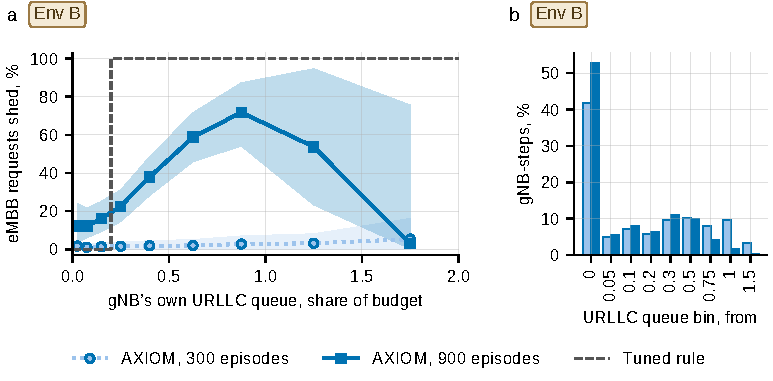
\includegraphics{figures/fig_decision.pdf}
\caption{What AXIOM learned in Env B at seven gNBs on the ring layout, 15 seeds. a, Share of gNB-steps on which its eMBB head would reject, by the gNB's own URLLC queue, with 95\% CIs over seeds. b, How often each queue level occurs}
\label{fig:s-decision}
\end{figure}

The distillation of the main paper's Section 6.3, M94, replays each stored checkpoint on its training and held-out streams, and the held-out replays reproduce the stored evaluations exactly. Each request gives four features, the gNB's URLLC queue, its congestion level, the requesting slice's PRB share, and the mean congestion of its neighbours. One tree per slice is fitted on training-stream decisions at the depth that 5-fold cross-validation selects, which was 3 for every target, and Table~\ref{tab:s-distil} gives the result. AXIOM rejected no URLLC request in any replay, and 34 of the 60 mMTC trees reject every request. The eMBB trees split first on the URLLC queue in 24 of 30 seeds at three gNBs, at a median of 0.21. At seven gNBs after 900 episodes they do so in 13 of 15 seeds, at a median of 0.28, against the tuned rule's 0.2.

\begin{table}[!htbp]
\caption{AXIOM distilled into one decision tree per slice in Env B. Fidelity is the share of held-out decisions on which the trees agree with AXIOM, by tree depth. The last columns run the depth-3 trees as a rule, with 95\% CIs and Holm-adjusted $p$}
\label{tab:s-distil}
\centering
\footnotesize
{\setlength{\tabcolsep}{3pt}
\begin{tabular}{@{}lcccccccc@{}}
\toprule
& & \multicolumn{3}{c}{Fidelity by depth} & \multicolumn{2}{c}{Rule minus AXIOM, reward} & \multicolumn{2}{c}{Rule minus tuned rule} \\
\cmidrule(lr){3-5}\cmidrule(lr){6-7}\cmidrule(l){8-9}
Checkpoints & Seeds & 1 & 2 & 3 & Difference & $p$ & Difference & $p$ \\
\midrule
3 gNBs, 300 episodes & 30 & 0.833 & 0.861 & 0.862 & $-$0.189 [$-$0.29, $-$0.09] & 0.0012 & $-$0.609 [$-$0.74, $-$0.47] & $<$0.001 \\
7 gNBs ring, 300 episodes & 15 & 0.963 & 0.964 & 0.974 & 0.057 [$-$0.54, 0.78] & 1 & $-$3.783 [$-$4.61, $-$2.91] & $<$0.001 \\
7 gNBs ring, 900 episodes & 15 & 0.927 & 0.925 & 0.931 & $-$0.147 [$-$0.29, 0.00] & 0.083 & $-$0.959 [$-$1.63, $-$0.40] & 0.0026 \\
\bottomrule
\end{tabular}}
\end{table}

\section*{S8. Throughput and delay}
Table~\ref{tab:s-kpi} lists throughput, the share of offered demand that is served, and delay, the mean backlog over the mean served PRBs in 5 s control periods, with the 95th percentile over steps and gNBs. This delay is a queueing proxy from the fluid model, not packet latency. Each re-run with a stored log reproduced it exactly, and the Env A accept-all rows, which have no stored log, are marked unchecked.

\begin{table}[!htbp]
\caption{Served share of offered demand and backlog delay in control periods, mean and 95th percentile, per slice}
\label{tab:s-kpi}
\centering
\scriptsize
\setlength{\tabcolsep}{2.5pt}
\begin{tabular}{lcccccc}
\toprule
Policy & URLLC served & eMBB served & URLLC delay & p95 & eMBB delay & p95 \\
\midrule
\multicolumn{7}{l}{Env A, three gNBs} \\
AXIOM & 99.8\% & 99.7\% & 0.11 & 0.66 & 0.11 & 0.47 \\
DQN-SA & 99.5\% & 99.4\% & 0.20 & 0.96 & 0.18 & 0.83 \\
DQN-I & 99.4\% & 98.5\% & 0.23 & 1.11 & 0.43 & 6.24 \\
MAPPO & 98.4\% & 90.5\% & 0.38 & 3.31 & 3.81 & 19.67 \\
Static rule & 99.8\% & 99.9\% & 0.10 & 0.59 & 0.05 & 0.31 \\
Accept all, unchecked & 97.5\% & 97.6\% & 0.80 & 3.01 & 0.76 & 2.65 \\
\midrule
\multicolumn{7}{l}{Env A, thirty-seven gNBs, hex} \\
AXIOM & 99.8\% & 99.0\% & 0.08 & 0.42 & 0.34 & 1.12 \\
DQN-SA & 94.2\% & 95.2\% & 3.61 & 16.87 & 2.09 & 14.28 \\
DQN-I & 97.7\% & 97.5\% & 0.76 & 5.23 & 0.72 & 5.49 \\
MAPPO & 96.4\% & 85.7\% & 0.58 & 5.38 & 6.28 & 35.70 \\
Static rule & 100.0\% & 100.0\% & 0.03 & 0.17 & 0.02 & 0.09 \\
Accept all, unchecked & 98.7\% & 98.8\% & 0.43 & 2.14 & 0.38 & 1.83 \\
\midrule
\multicolumn{7}{l}{Env B, three gNBs} \\
AXIOM & 98.4\% & 88.5\% & 0.65 & 2.32 & 3.18 & 19.28 \\
DQN-SA & 98.2\% & 82.1\% & 0.75 & 3.15 & 5.73 & 49.79 \\
DQN-I & 98.6\% & 82.7\% & 0.66 & 2.81 & 4.73 & 49.34 \\
MAPPO & 97.2\% & 83.5\% & 1.10 & 4.00 & 4.57 & 43.82 \\
Static rule & 96.0\% & 96.1\% & 1.59 & 5.25 & 1.57 & 5.11 \\
Tuned rule & 99.0\% & 84.8\% & 0.58 & 1.96 & 3.57 & 38.55 \\
Accept all & 92.8\% & 92.9\% & 2.59 & 7.72 & 2.58 & 7.59 \\
\midrule
\multicolumn{7}{l}{Env B, nineteen gNBs, hex} \\
AXIOM & 96.6\% & 92.6\% & 1.35 & 4.67 & 3.41 & 16.01 \\
DQN-SA & 93.8\% & 93.9\% & 2.26 & 6.99 & 2.24 & 6.82 \\
DQN-I & 94.1\% & 86.1\% & 2.17 & 9.71 & 4.17 & 72.77 \\
MAPPO & 89.2\% & 88.3\% & 2.66 & 33.84 & 2.58 & 28.13 \\
Static rule & 96.8\% & 96.9\% & 1.33 & 4.65 & 1.32 & 4.50 \\
Tuned rule, carried & 99.1\% & 87.9\% & 0.51 & 1.77 & 2.78 & 25.40 \\
Accept all & 93.8\% & 93.9\% & 2.25 & 6.97 & 2.24 & 6.82 \\
\bottomrule
\end{tabular}
\end{table}

\section*{S9. Reproducing the results}
Fig.~\ref{fig:repro} sets out what reproducing the results needs and the order of the steps. Every result in both documents comes from one laptop without a graphics processor, and every simulation run fixes its seed.

\begin{figure}[!htbp]
\centering
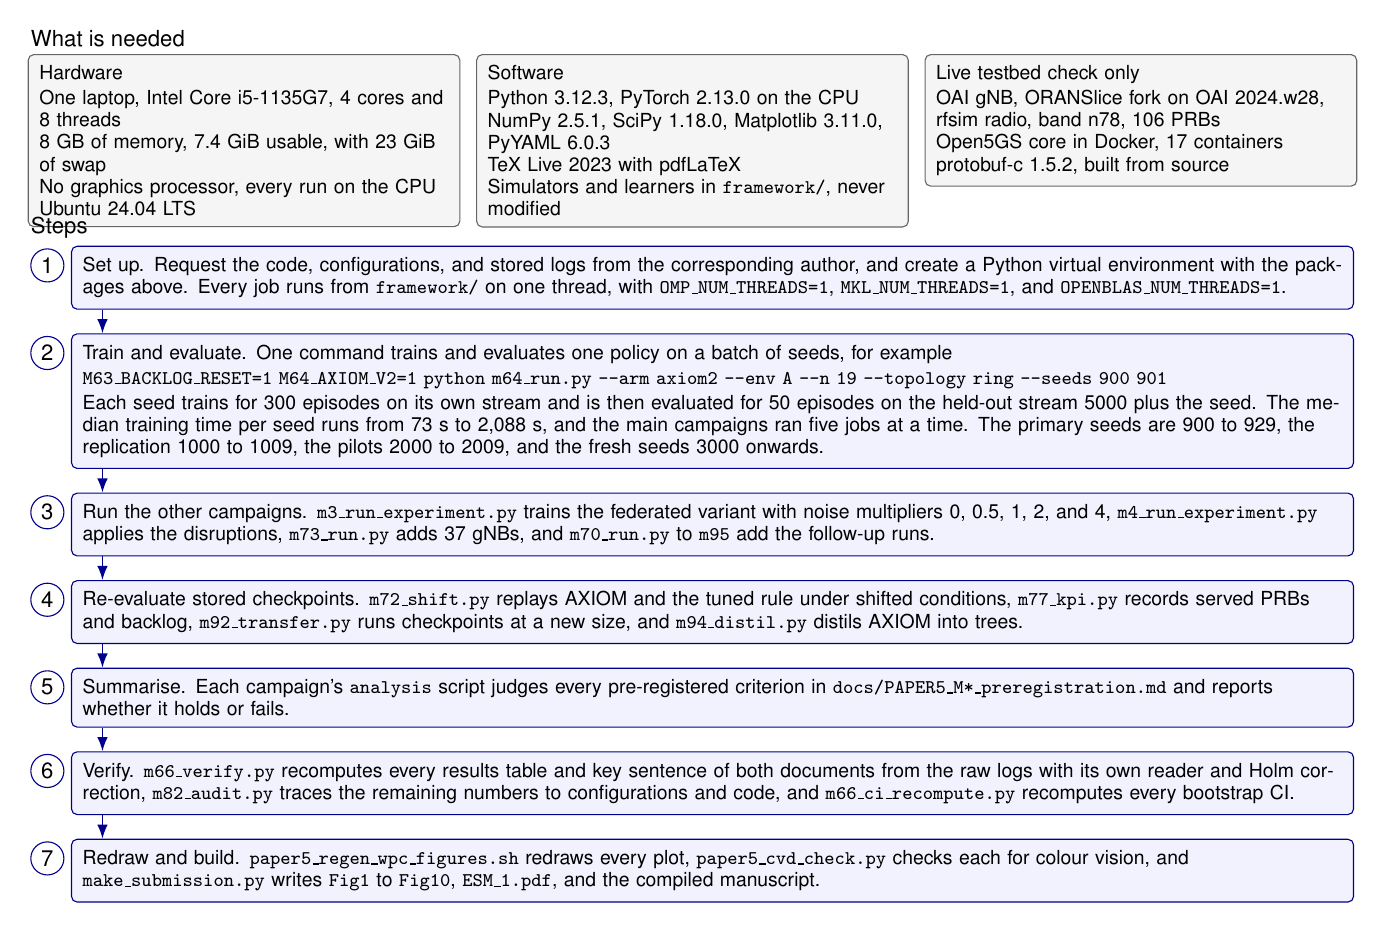
\begin{tikzpicture}[
  font=\fontfamily{phv}\selectfont\scriptsize,
  need/.style={draw=black!60, rounded corners=2pt, fill=gray!8, align=left, text width=5.2cm, inner sep=4pt, anchor=north west},
  stp/.style={draw=blue!55!black, rounded corners=2pt, fill=blue!5, align=left, text width=16.0cm, inner sep=4pt, anchor=north west},
  liv/.style={draw=orange!75!black, rounded corners=2pt, fill=orange!8, align=left, text width=16.0cm, inner sep=4pt, anchor=north west},
  num/.style={circle, draw=blue!55!black, fill=white, inner sep=1pt, minimum size=0.42cm, font=\fontfamily{phv}\selectfont\footnotesize},
  hd/.style={font=\fontfamily{phv}\selectfont\footnotesize, anchor=south west, inner sep=1pt},
  tt/.style={font=\ttfamily\footnotesize},
  ar/.style={-{Latex[length=1.8mm]}, semithick, blue!55!black}
]
\newcommand{\bt}[1]{{\fontfamily{phv}\selectfont #1}}
% what is needed
\node[need] (hw) at (0,0) {\bt{Hardware}\\[1pt]
  One laptop, Intel Core i5-1135G7, 4 cores and 8 threads\\
  8 GB of memory, 7.4 GiB usable, with 23 GiB of swap\\
  No graphics processor, every run on the CPU\\
  Ubuntu 24.04 LTS};
\node[need] (sw) at ($(hw.north east)+(0.2,0)$) {\bt{Software}\\[1pt]
  Python 3.12.3, PyTorch 2.13.0 on the CPU\\
  NumPy 2.5.1, SciPy 1.18.0, Matplotlib 3.11.0, PyYAML 6.0.3\\
  TeX Live 2023 with pdfLaTeX\\
  Simulators and learners in \texttt{framework/}, never modified};
\node[need] (lv) at ($(sw.north east)+(0.2,0)$) {\bt{Live testbed check only}\\[1pt]
  OAI gNB, ORANSlice fork on OAI 2024.w28, rfsim radio, band n78, 106 PRBs\\
  Open5GS core in Docker, 17 containers\\
  protobuf-c 1.5.2, built from source};
\node[hd] at ($(hw.north west)+(0,0.05)$) {What is needed};
% steps
\node[stp] (s1) at ($(hw.west |- lv.south)+(0.55,-0.75)$) {\bt{Set up.} Request the code, configurations, and stored logs from the corresponding author, and create a Python virtual environment with the packages above. Every job runs from \texttt{framework/} on one thread, with \texttt{OMP\_NUM\_THREADS=1}, \texttt{MKL\_NUM\_THREADS=1}, and \texttt{OPENBLAS\_NUM\_THREADS=1}.};
\node[stp] (s2) at ($(s1.south west)+(0,-0.3)$) {\bt{Train and evaluate.} One command trains and evaluates one policy on a batch of seeds, for example\\[1pt]
  \texttt{M63\_BACKLOG\_RESET=1 M64\_AXIOM\_V2=1 python m64\_run.py -{}-arm axiom2 -{}-env A -{}-n 19 -{}-topology ring -{}-seeds 900 901}\\[1pt]
  Each seed trains for 300 episodes on its own stream and is then evaluated for 50 episodes on the held-out stream 5000 plus the seed. The median training time per seed runs from 73 s to 2{,}088 s, and the main campaigns ran five jobs at a time. The primary seeds are 900 to 929, the replication 1000 to 1009, the pilots 2000 to 2009, and the fresh seeds 3000 onwards.};
\node[stp] (s3) at ($(s2.south west)+(0,-0.3)$) {\bt{Run the other campaigns.} \texttt{m3\_run\_experiment.py} trains the federated variant with noise multipliers 0, 0.5, 1, 2, and 4, \texttt{m4\_run\_experiment.py} applies the disruptions, \texttt{m73\_run.py} adds 37 gNBs, and \texttt{m70\_run.py} to \texttt{m95} add the follow-up runs.};
\node[stp] (s4) at ($(s3.south west)+(0,-0.3)$) {\bt{Re-evaluate stored checkpoints.} \texttt{m72\_shift.py} replays AXIOM and the tuned rule under shifted conditions, \texttt{m77\_kpi.py} records served PRBs and backlog, \texttt{m92\_transfer.py} runs checkpoints at a new size, and \texttt{m94\_distil.py} distils AXIOM into trees.};
\node[stp] (s5) at ($(s4.south west)+(0,-0.3)$) {\bt{Summarise.} Each campaign's \texttt{analysis} script judges every pre-registered criterion in \texttt{docs/PAPER5\_M*\_preregistration.md} and reports whether it holds or fails.};
\node[stp] (s6) at ($(s5.south west)+(0,-0.3)$) {\bt{Verify.} \texttt{m66\_verify.py} recomputes every results table and key sentence of both documents from the raw logs with its own reader and Holm correction, \texttt{m82\_audit.py} traces the remaining numbers to configurations and code, and \texttt{m66\_ci\_recompute.py} recomputes every bootstrap CI.};
\node[stp] (s7) at ($(s6.south west)+(0,-0.3)$) {\bt{Redraw and build.} \texttt{paper5\_regen\_wpc\_figures.sh} redraws every plot, \texttt{paper5\_cvd\_check.py} checks each for colour vision, and \texttt{make\_submission.py} writes \texttt{Fig1} to \texttt{Fig10}, \texttt{ESM\_1.pdf}, and the compiled manuscript.};
\node[hd] at ($(s1.north west)+(-0.55,0.05)$) {Steps};
\foreach \i/\j in {s1/s2,s2/s3,s3/s4,s4/s5,s5/s6,s6/s7}{\draw[ar] ($(\i.south west)+(0.4,0)$) -- ($(\j.north west)+(0.4,0)$);}
\foreach \i [count=\k] in {s1,s2,s3,s4,s5,s6,s7}{\node[num] at ($(\i.north west)+(-0.3,-0.25)$) {\k};}
\end{tikzpicture}
\caption{Reproducing the results. Top, the hardware and software every run used. Below, the steps from the stored code to the figures and the manuscript, with the live testbed in Section S3}
\label{fig:repro}
\end{figure}

\end{document}
